\documentclass[a4paper,12pt]{article}

% For \url
\usepackage{hyperref}

% For line skip paragraphs
\usepackage[parfill]{parskip}

% For smaller margins
\usepackage[margin=1in]{geometry}

% For images
\usepackage{graphicx}
\usepackage{caption}
\usepackage{subcaption}

%For align environment
\usepackage{amsmath}

% For UTF-8
\usepackage[utf8]{inputenc}

% For verbatim environment
\usepackage{verbatim}

% Set section numbering to Roman
\renewcommand \thesection{\Roman{section}}
\renewcommand \thesubsection{\arabic{section}.\arabic{subsection}}

\title{TDT4258 \\ Energy Efficient Computer Design \\ Exercise 2}
\author{
    Lundal, Per Thomas \\ \texttt{perthol@stud.ntnu.no}
    \and
    Normann, Kristian \\ \texttt{krinorm@stud.ntnu.no}
    \and
    Selvik, Andreas Løve \\ \texttt{andrels@stud.ntnu.no}
}
\date{\today}

\begin{document}
\maketitle
\begin{abstract}

This report presents a MIDI player implemented on an AVR32 microcontroller\cite{avr32}. This is the result of assignment 2 given in TDT4258, for which the requirements are to make a program that allows one to play different sound effects by pushing buttons on the STK1000. It is done by first parsing the MIDI files into a simpler intermediate event-based format which can be played efficiently by the STK1000.

\end{abstract}

\newpage
\tableofcontents

\clearpage
\section{Introduction}
Our focus for this assignment was to generate as smooth a sound as possible. As opposed to the previous assignment, this time around we did not give much thought to energy efficiency and tried instead to make sure the resulting music would be able to make use of as many tones as possible without loss of notable speed, while also minimizing background noise.

Physically, sound is longitudinal waves that propagate through a medium, often the air. Which means that we have to produce waves, and that gives us the properties of waves to work with; frequency, amplitude, waveform and interference. Frequency is the property that decides the perceived pitch of the sound and amplitude, see figure \ref{sinwave}, decides the loudness. The waveform, see figure \ref{waveforms}, has impact on multiple aspects of the sound, the most prominent being that the average amplitude is higher and thereby sound produced will be louder, it also changes sounds characteristics. When there is multiple sounds, that is, basic harmonic waves, at the same time they interfere, which gives the result of the amplitude in a given point being the sum of the amplitude in all the waves in that point. 

To produce sound digitally, one has to be able to generate samples. A sample is the numerical value of the current wave amplitude in a point, see figure \ref{digwave}. In order to capture the frequency of the intended wave, the frequency of the samples has to be at least twice the maximum frequency of the sound produced. Humans are capable of perceiving sound with a frequency between 20Hz and 20kHz, so in order to produce the whole range we would need a sample rate above 40kHz. As we’ll see, we have a sample rate of 23.4kHz, which means that we can produce sound with a maximum frequency of 11.7kHz. 

The STK1000 is equipped with an Audio Bitstream Digital Analog Converter
(ABDAC) that handles these samples. It functions such that the user has to feed it a consistent stream of 16 bit samples, which it then turns into an analog electrical signal that is sent to a speaker. Here, the electrical signal will move a magnet connected to a membrane: generating sound waves.

By hooking an interrupt routine up with a clock, we were able to deliver samples to the ABDAC at a consistent rate.

Our note system is a set of 12 notes evenly spaced. Mathematically this spacing is 
\begin{align*}
f_0&=233\\
f_n&=\sqrt[12]{2} * f_{n-1}
\end{align*} 
where $f_n$ is the frequency of the n-th note. The set of 12 consecutive notes is called an octave. The next octave on a note is obtained by multiplying the frequency by 2. 

MIDI is a sound format that generates sounds by turning off and on different notes from different channels. It uses events which specifies which note to turn on and off at what time. The final sound samples are produced by summing the samples of each channel. 

\begin{figure}[b]
        \centering
        \begin{subfigure}[b]{0.57\textwidth}
                \centering
                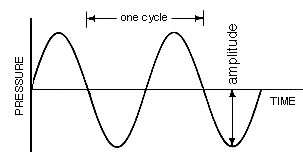
\includegraphics[width=\textwidth]{sinwave}
                \caption{A wave\cite{sinewave}.}
                \label{sinwave}
        \end{subfigure}%
        ~ 
        \begin{subfigure}[b]{0.52\textwidth}
                \centering
                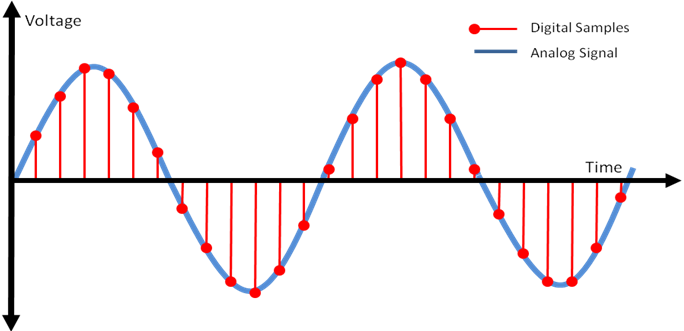
\includegraphics[width=\textwidth]{digwave}
                \caption{Samples of a wave\cite{samples}.}
                \label{digwave}
        \end{subfigure}
    \caption{Sound waves}
   \label{waves}
\end{figure}
\begin{figure}[b]
        \centering
            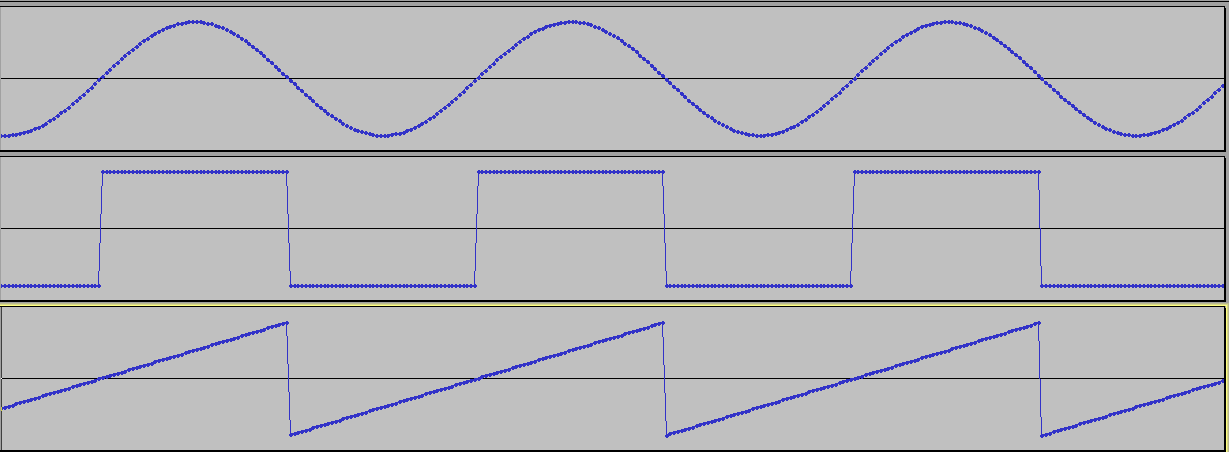
\includegraphics[width=\textwidth]{waveforms}
            \caption{Different waveform in audacity. From top to bottom: sine, square and jagged wave.}
            \label{waveforms}
\end{figure}



\clearpage
\section{Description And Methodology}

The assignment was solved in the following steps:
\begin{enumerate}
\item Implement the first assignment in C
\item Generate noise with the ABDAC
\item Generate tones with different wave types and frequencies
\item Play MIDI tunes
\end{enumerate} 

\subsubsection*{Jumper and cable configuration}
\begin{itemize}
\item The LED’s were connected to PIOC by a flat-cable from GPIO pins 16-23(J3) to the LED-pins(J15) on the STK1000 board \cite[section~2.4.1]{compendium}.
\item The buttons were connected to PIOB by flat-cable from GPIO pins 0-7(J1) to the SWITCH-pins(J25) on the STK1000 board \cite[section~2.4.1]{compendium}.
\item On the AT32AP7000 we set the jumpers SW6 and SW4 to GPIO(so that PIOC and PIOB would be connected to GPIO)\cite[table~2.3]{compendium}.
\end{itemize}

\subsection{LEDs and Buttons}

The LEDs and buttons were to be operated in a similar manner as in Assignment 1. However, as it now was to be written in C, the method of accessing the registers was a bit different. The AVR32 C libraries makes these available through a number of simple structs though, so the main difference was the syntax. The code for initialization can be seen below:

\begin{verbatim}
// Initialize the buttons
register_interrupt(button_isr, AVR32_PIOB_IRQ / 32, AVR32_PIOB_IRQ % 32, BUTTONS_INT_LEVEL);
piob->per = 0xFF;
piob->puer = 0xFF;
piob->ier = 0xFF;

// Initialize the LEDs
pioc->per = 0xFF;
pioc->oer = 0xFF;
pioc->codr = 0xFF;
\end{verbatim}

The interrupt routine was implemented by first debouncing, then determining what button was pressed by looking at the ISR (Interrupt Status Register) and PDSR (Pin Data Status Register), and finally updating the lights by writing to SODR (Set Output Data Register) and CODR (Clear Output Data Register).

\subsection{ABDAC}

Once the LEDs were shining and reacting to the buttons, the next objective was enabling the ABDAC. By following the procedure in the compendium \cite{compendium}, we started by releasing the
ABDAC pins (20 and 21) from PIOB by writing 1 to its PDR (Pin Disable Registers) and followed by connecting them to Peripheral A (ABDAC) by writing to it’s A Select Register (ASR). The procedure for enabling the clock was not described in the compendium, so for this we searched for an example on the internet. There we found the code file for an AVR32 MP3 player \cite{clockex} which led us to the following code for using oscillator 1:

\begin{verbatim}
pm->GCCTRL[6].pllsel = 0;
pm->GCCTRL[6].oscsel = 1;
pm->GCCTRL[6].cen = 1;
\end{verbatim}

Finally we activated the ABDAC by writing 1 to its enable bit in CR (Control Register) and set the interrupt routine to write random data to SDR (Set Data Register). This made the board output white noise, which meant we could proceed to generating some tones.

\subsection{Tones}

At the the beginning of the main method we initialize a set of twelve notes (an octave) corresponding to the wave type parameter given to the tones initialization function. The notes are built from this wave type and and a given, hardcoded frequency. Each note is an oscillation variable computed by multiplying the sample\_amplitude with some value corresponding the the wave type. $A * f$, (where A is the amplitude, f is the wave type function).

\subsection{MIDI}

With the ability to play different tones and the desire to play some sweet tunes in mind, we decided to implement a system for playing MIDI files. Since the raw MIDI format is not especially well designed for playback on the board, and we would like to play as many simultaneous tones as possible, it was decided to create a simplified format. In addition, some means to pass the data to the board and access it was required. This was accomplished by designing a set of structs to hold the data:

\begin{verbatim}\label{midi_event}
typedef struct {
    int32_t delta_time;
    int8_t channel;
    int8_t tone;
    int8_t volume;
} midi_event_t;

typedef struct {
    int32_t num_events;
    midi_event_t events[];
} midi_soundtrack_t;
\end{verbatim}

This solution uses 7 bytes of data for each event, which is slightly more than the average for MIDI. In addition, it only supports up to 128 simultaneous tones (opposed to the 4096 of MIDI), and does not take instrument types into account. But there is only one stream of events compared to the possible $2^(16)$ of MIDI, which makes it much easier to process for the board.

Next up was the playback system. It was needed to keep track of all playing tones and their volume. Additionally, we didn’t want to create different samples for all 128 tones as this would require a lot of memory. Therefore we also needed to keep track of the pitch shift which essentially changes the playback speed. This was accomplished by creating yet another struct:

\begin{verbatim}
typedef struct {
    sample_t *sample;
    int32_t sample_point;
    int8_t pitch_up;
    int8_t pitch_down;
    int8_t volume;
} midi_channel_t;
\end{verbatim}

The reason for both pitch\_up and pitch\_down instead of a single variable for pitch\_shift is so that we avoid an if-test in the playback procedure to determine the shift direction, which in turn allows us to play more tones simultaneously. A single global variable is used to keep track of the current soundtrack.

Now we could focus on the main playback procedure midi\_tick(), which is to be called once for each ABDAC interrupt and return the next output value. We started by implementing the event processing. For this we needed to keep track of the next event and the time passed since last event, which we stored in global variables. Then, on each call the time passed is compared to the next event’s delta\_time. If it is greater, then it sets a new sample, pitch and volume for a channel as specified by the event. Afterwards, it prepares for processing the next event by resetting the time passed and updating the next event counter. The tone and pitch is calculated as in the following pseudocode:

\begin{verbatim}
// Retrieve tone and pitch
sample = event.tone  % 12;
pitch = event.tone / 12;
\end{verbatim}

After processing events, the time is incremented. Then it advances and pulls output data from all channels by calling mid\_channel\_advance() for each of them. The output is summed and then normalized by dividing by 128, which is the maximum MIDI volume, and the number of channels. This ensures that the final output signal will have the same maximum amplitude as the individual samples.

The method responsible for advancing each channel is midi\_channel\_advance(). It works by simply retrieving the sample point for that channel’s sample and adjusting it for volume. Then it calculates how far it should advance in the sample depending on what pitch it is being played on. For each pitch up it should play twice as fast, and thus advance twice as many sample points. Then it advances using an modulo operation to wrap around to the beginning. One thing to note is that the samples generated by tones\_init() are of pitch 5, and thus calculations has to be compensated for it by shifting.

With the midi playback system in order, all that remained to get sound output was to create a loop in the main function that calls midi\_tick() and updates a global variable with the returned value, before sleeping until awoken by the next ABDAC interrupt. The overall program flow can be seen in figure \ref{progflow} and \ref{interrupt}.

\begin{figure}
        \centering
        \begin{subfigure}[b]{0.57\textwidth}
                \centering
                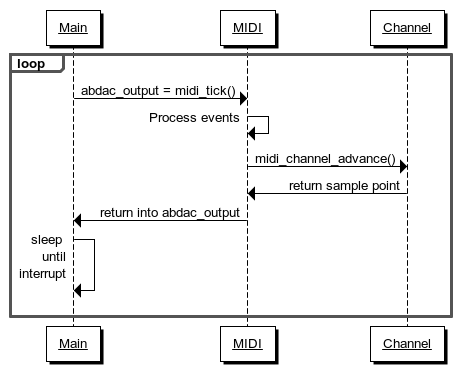
\includegraphics[width=\textwidth]{progflow}
                \caption{The main loop}
                \label{mainloop}
        \end{subfigure}%
        ~ 
        \begin{subfigure}[b]{0.52\textwidth}
                \centering
                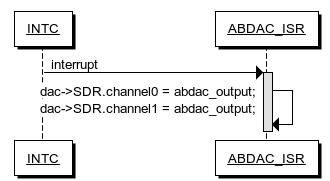
\includegraphics[width=\textwidth]{interrupt}
                \caption{The interrupt routine}
                \label{interrupt}
        \end{subfigure}
      \caption{Overview of the system}
   \label{progflow}
\end{figure}
\subsection{MIDI Converter}

With the setup functioning correctly, verified by some simple test soundtracks, the time had come to make a program that converts the MIDI files to our simplified format. This was perhaps the most challenging part of the assignment. The first step was to find good documentation of the MIDI file format. The one we found to be most useful and descriptive was an online guide by The Sonic Spot \cite{sonicspot}. With this knowledge in hand, the work started.

Since MIDI is structured like a buffer, we started by reading the whole MIDI file into one. This allowed us to create a few simple methods to get the next value from the file, parse\_varint() and parse\_int(). The first reads a variable-length number where the most significant bit of each byte determines whether it should continue or not. The second reads a specified number of bytes.

We started the parsing by first reading the header data followed by storing the individual tracks into different buffers. Since the board can only play so many tones at a time, we also created a global variable to to keep track of how many of the channels were in use. We then continued to the main processing loop.

Since our simplified format only has one sequence of events, it is necessary to merge all the MIDI tracks into one. This was accomplished by checking the delta-time of the next event for each track to determine the which one had the soonest event. Once we have found the track, we process the next event on it by calling track\_process\_event(), before updating the delta-times of the other tracks to make sure everything stays in sync.

We process the next event by first checking its type. Due to our simplified format we only cared about a few of them, namely “Note on”, “Note off” and “Set tempo”. The rest still had to be taken into account though, as we needed to skip the correct amount of bytes.

For note on events it was necessary to find an available channel. This was done with the function channel\_find() which checks all channels for one that is available. However, if none is found and the parameter to enforce channel stealing is enabled, it will return the channel with lowest volume. This allows playback of MIDI files with more concurrent tones while reducing sound artifacts. For note off events we call the function channel\_recover() which simply sets the channel to unused. If it is not found, either due to an error in the MIDI file or channel stealing, it will produce a warning.

Then, for both event types, we output data for one event of our simplified format. Delta-time is saved as the number of seconds multiplied by the sample rate (example: 0.31 * SAMPLE\_RATE) to increase portability, and allow us to change the playback sample rate without reconverting the MIDI files. Set tempo only triggers a recalculation of the global BPM (Beats Per Minute) variable.

Only the note on and off events consumes time in our format. This meant that the delta-time of other events had to be added to the next event of that track. This was accomplished by returning 1 for those that consume time and 0 for those that do not, which the main loop uses to update the times. This concluded our converter, and the whole MIDI system was complete. The general program flow for the converter can be seen in figure \ref{midi2c}.

\begin{figure}[b]
        \centering
            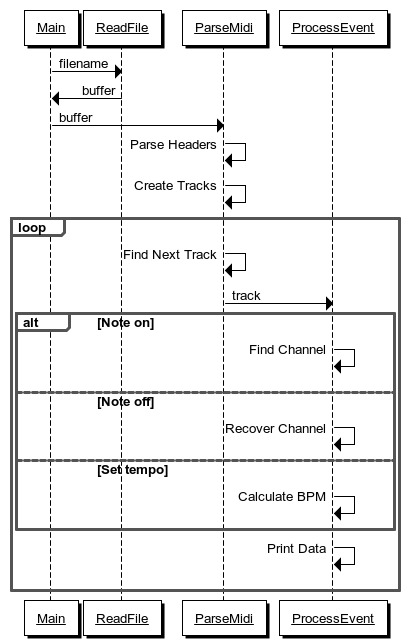
\includegraphics[width=\textwidth]{midi2c}
            \caption{MIDI converter}
            \label{midi2c}
\end{figure}

\subsection{Tools}

\begin{itemize}
\item Audacity for observing and measuring sound output and waveforms
\item GitHub for handling version control
\item Vim as main code-editor
\item Google Docs for report collaboration
\item \LaTeX for report markup
\item JTAGICE mkII for connecting the computer to the board
\item avr32gdbproxy for connecting to JTAGICE mkII
\item avr32-gdb for connecting to the board, allowing us to debug the code
\item \url{www.websequencediagrams.com} for drawing sequence diagrams
\end{itemize}

\clearpage
\section{Results And Tests}
We designed some tests for the final implementation, see Appendix A. The final version passed all of these tests, save one instance during development. The  “Two interleaving button-clicks” test failed when including button SW0 in the test. As it turned out, this was because the ‘debounce-loop’ was removed in optimization by the compiler. This was fixed by making the debounce-variable volatile. After this all tests worked without fault.

\clearpage
\section{Evaluation Of Assignment}
It was a fun challenge!

It was however a bit difficult to understand how to enable the clock for the ABDAC, as the only reference in the Compendium \cite{compendium} is the line “pm\rightarrow GCCTRL[6] = data”.

\clearpage
\section{Discussion}

During the startup phase, after turning on the STK1000, just before LED0 is lit and its corresponding music starts to play, some random light-arrangement occurs based on what is present in memory from previous. This does not interfere with any expected functionality.      

During development we noticed a strong audible difference between square waves and sine waves, see figure \ref{waveforms}. We heard the sounds generated with square waves much clearer than the sine waves and elected therefore to use them for our final code, even though it sounded more electronic, so to speak.

We did observe in Audacity however that the sound output isn’t quite what we expected. Sine waves look correct, but square waves does not look square, as can be seen in figure \ref{actualsquare}. We do not know if this is because of hardware deterioration, or simply the inner workings of the ABDAC.
\subsection{Issues}

At one point during development, we noticed that with eight tracks enabled, we could play two tracks simultaneously without loss of speed and clarity of sound (i.e no particularly greater amount of crackling, or noise in the background). Any more tracks played at the same time however, would result in slower and more faded sound. This was discovered to be due to the ABDAC underrunning, causing it to use an extra interrupt cycle, and thus reducing the pitch.

After some inquiries we came upon a stackoverflow post\cite{multifile}, which stated that having multiple source files(which we do), decreased run-time performance. We then made an “all” c file that included all the c files and compiled this “all” file. We are inclined to believe that the post’s claim was correct as doing this let us play a whole eight tracks without loss of speed.

A problem that has continued through the whole assignment is noise from the ABDAC. During pauses in the music, where the ABDAC is fed the value 0 repeatedly, a tone with seemingly random frequency can be heard. All attempts at correcting this in software have only masked the problem by another sound and thus failed. However, by intense searching of the internet we found that the audio output of the STK1000 might not be designed for load-heavy devices such as headphones, and that it might sound better when connected to an amplifier\cite{impedance}. By connecting the output to some speakers we noticed a slight reduction in the noise level, but it was still present. This leads us to think it is a hardware issue that we can not prevent. 

Oscillator division seems not to be working according to specifications. At first we just made the playback system think it was running at a lower sample rate and then made the ABDAC constantly underrun (So that the abdac only received data every other interrupt cycle). We did however, find out that it does work if we enable clock division after enabling the clock. This is the exact opposite from the recommended procedure in the AP7000 documentation \cite{ap7000}.

The MIDI format allows for theoretically up to 2048 notes to be played simultaneously. However, when running our code, the STK1000 could only play 12 simultaneous notes at approximately 24 kHz. If we try to increase the number of notes we’ll have to decrease the frequency and vica versa.

It’s worth noting that MIDI files don’t always follow the standard. Sometimes they use note on events with volume 0 instead of note off, note on events instead of note aftertouches and so on. In addition, a relatively vital part of the specification was left out by what sources we could find \cite{sonicspot} \cite{mididoc}. This is that when the most significant bit of the type-and-channel byte (first byte after delta-time) is 0, this is actually the first parameter to the event, and the type-and-channel is that of the previous event. This is possible because all type-and-channel bytes have a most significant bit of 1 and parameters 0. This complicated the development of the MIDI converter.


\subsection{Modularity}

The modularity of the code was central during the development, as it is important to be able to reuse the code for later assignment and whenever we need midi sound on some system. Therefore we tried to keep most of the code general, and the only hardware specific code should be in oeving2.c. This means that it shouldn’t pose a great challenge to use this code to produce sound with an operating system and drivers. There are some hardcoded values however, like the sample rate, that is defined specifically instead of taken as an argument, but this was a deliberate compromise for code speed over modularity. Furthermore, the midi initialization routine could have taken \emph{number of channels} as an argument, but we have elected not to allow for this. The reasons are that this would interfere with the compiler’s loop unrolling optimization, which in turn would lead to if-tests, branching, a chance of pipeline bubbles and in effect, slower execution.


\clearpage
\section{Conclusion}
In the end we did not only have a system that satisfied the requirements, but a full-fledged MIDI player. This gives us a great deal of flexibility when we are to implement the game in the next exercise. It leaves us free to choose from a virtually infinite supply of free midi files all over the internet.
We have gained insight into writing C code without an operating system, and learned how to use I/O and interrupts in C. Furthermore we managed to use the microcontroller’s ABDAC to play our self-converted MIDI files.

\clearpage

\begin{thebibliography}{9}

\bibitem{compendium}
Computer Architecture and Design Group,
\emph{Lab Assignments in TDT4258 Energy Efficient Computer Systems}.
Department of Computer and Information Science, NTNU,
2013,
\url{http://www.idi.ntnu.no/emner/tdt4258/\_media/kompendium.pdf}.

\bibitem{avr32}
Atmel.
\emph{AVR32 Architecture Document},
2011,
\url{http://www.idi.ntnu.no/emner/tdt4258/\_media/doc32000.pdf}.

\bibitem{ap7000}
Atmel.
\emph{AT32AP7000 Preliminary},
2009,
\url{http://www.idi.ntnu.no/emner/tdt4258/\_media/doc32003.pdf}.

\bibitem{clockex}
Atmel. “abdac.c”
\emph{asf.atmel.com},
Web.09.03.2013.
\textless \url{http://asf.atmel.com/docs/latest/avr32.applications.audio-player.mp3.evk1104/html/abdac_8c_source.html}
\textgreater

\bibitem{impedance}
AVR32
\emph{avrfreaks.net},
Web 09.03.2013,
\textless
\url{http://www.avrfreaks.net/index.php?name=PNphpBB2&file=printview&t=53711&start=0}
\textgreater

\bibitem{sonicspot}
Sonicspot, “MIDI File Format”
\emph{sonicspot.com}
Web 14.03.2013
\textless
\url{http://www.sonicspot.com/guide/midifiles.html}
\textgreater

\bibitem{mididoc}
cse4501, “The MIDI File Format”
\emph{cse4051/projects/midi}
Web 14.03.2013
\textless
\url{http://cs.fit.edu/~ryan/cse4051/projects/midi/midi.html}
\textgreater




\bibitem{multifile}
“Multiple source file executable slower than single source file executable“, 
\emph{stackoverflow.com}
17.03.2012 Web 14.03.2013
\textless
\url{http://stackoverflow.com/questions/9742934/multiple-source-file-executable-slower-than-single-source-file-executable}
\textgreater

\bibitem{samples}
\emph{projeneering.com}
\textless
\url{http://projeneering.com/technical_articles/images_pid_primer/sampling.png}
\textgreater

\bibitem{sinewave}
Simon Fraser University “Sine Wave.gif”
\emph{sfu.ca}
\textless
\url{http://www.sfu.ca/sonic-studio/handbook/Graphics/Sine_Wave.gif}
\textgreater
\end{thebibliography}

\clearpage
\appendix
\addcontentsline{toc}{section}{Appendix}
\section{Tests}

\begin{tabular}[h]{|lp{12cm}|} \hline
\textbf{\emph{Test 1:}} 		& \textbf{Starting the machine}\\
\emph{Action:} 		& Turn on the STK1000\\
\emph{Preconditions:}	& Uploaded program on microcontroller and power cable is connected\\
\emph{Wanted outcome:}	& LED0 should light up and 'Under pressure' should play. \\ \hline
\end{tabular}
\vspace{1cm}

\begin{tabular}[h]{|lp{12cm}|} \hline
\textbf{\emph{Test 2:}} 		& \textbf{Switch song}\\
\emph{Action:} 		& Press button SW X\\
\emph{Preconditions:}	& LED Y lit and the music corresponding to SW Y should be playing.\\
\emph{Wanted outcome:}	& LED Y turns off and LED X turns on. Music corresponding to SW Y stops and the music corresponding to SW X starts from the beginning.\\ \hline
\end{tabular}
\vspace{1cm}

\begin{tabular}[h]{|lp{12cm}|} \hline
\textbf{\emph{Test 3:}} 		& \textbf{One click, one action}\\
\emph{Action:} 		& Wait two seconds and release the button.\\
\emph{Preconditions:}	& Press button SW X and hear the music start playing.\\
\emph{Wanted outcome:}	& Upon releasing the button, the music should continue and not start over. \\ \hline
\end{tabular}
\vspace{1cm}

\begin{tabular}[h]{|lp{12cm}|} \hline
\textbf{\emph{Test 4:}} 		& \textbf{Two interleaving button-clicks}\\
\emph{Action:} 		& First press button SW X and hold it, press press button SW Y (where $X \neq Y$), release button SW X and finally, release button SW Y. \\
\emph{Preconditions:}	& The board is turned on and some LED Z is lit with its corresponding music playing.\\
\emph{Wanted outcome:}	& Upon pressing button SW X, its corresponding music begins to play. Then, SW Y is pressed, the music changes to button SW Y's corresponding music. When button SW X is released, it changes nothing and the music continues to play, and lastly, when button SW Y is released, nothing changes and the music continues to play uninterrupted. \\ \hline
\end{tabular}
\vspace{1cm}

\begin{tabular}[h]{|lp{12cm}|} \hline
\textbf{\emph{Test 5:}} 		& \textbf{Quick click}\\
\emph{Action:} 		& Press button SW Y 5 times with 1-second intervals.\\
\emph{Preconditions:}	& The board is turned on and some LED X is lit with its corresponding music playing.\\
\emph{Wanted outcome:}	& LED Y lights up and stays lit upon the first pressing of the button, and the music corresponding to button SW Y starts over each time the button is pressed.\\ \hline
\end{tabular}

\end{document}
